%% Copyright (C) 2019 Turysaz, Bitbonk
\documentclass{beamer}

%% Copyright (C) 2019 Turysaz, Bitbonk

\usepackage[utf8]{inputenc}
\usepackage[T1]{fontenc}
\usepackage[english]{babel}

\usepackage{todonotes}

%% packages needed by DarkConsole theme
\usepackage{xcolor}
\usepackage{pgf}
\usepackage{droidsans}
\usepackage{fvextra}
\usepackage{upquote}
\usepackage{slantsc}
%\usepackage{minted} %% needs shell escaping...
%\usepackage{ifplatform} %% needs shell escaping...
\usepackage{xstring}
\usepackage{framed}

\usetheme{DarkConsole}

\usepackage{pdfpcnotes}

\usepackage{caption}
\captionsetup[figure]{labelformat=empty}

\newcommand{
    \emojiLarge}[1]{
    \includegraphics[width=2cm]{../3rd-party/coloremoji/emoji_images/hires/#1.pdf}}

\newcommand{
    \emojiMedium}[1]{
    \includegraphics[width=1cm]{../3rd-party/coloremoji/emoji_images/hires/#1.pdf}}


\newcommand{
    \emojiSmall}[1]{
    \includegraphics{../3rd-party/coloremoji/emoji_images/hires/#1.pdf}}

\newcommand{\emojiCheck}{\emojiSmall{2705}}
\newcommand{\emojiFail}{\emojiSmall{1F6AB}}

%\newcommand{\says}[1]{\note{\huge{Says: \alert{#1}}}}
\newcommand{\says}[1]{\pnote{Says: #1}}



%% variables for koma title page
\author{\{@turysaz, @bitbonk\}}
\title{\Huge{Knit Rider}\\
    \large{Bring that 80s knitting machine to the 21st century!}
}
\date{\today{}}

\begin{document}

\maketitle

\begin{frame}{init}
    \begin{itemize}[<+->]
        \item We had an old knitting machine
        \item It looked cool
        \item It \alt<+>{\alert{had}}{seemed to have} a data interface
              \only<.>{\alert{\textbackslash{}o/}}
    \end{itemize}
\end{frame}

\begin{frame}{the idea}
    \begin{enumerate}[<+->]
        \item Take a photo!
        \item Image processing!
        \item Do \_all\_ the soldering!
        \item Speak the protocol!
        \item Knit your face!
    \end{enumerate}
\end{frame}

\begin{frame}{the brother kh-940}
    \begin{figure}
        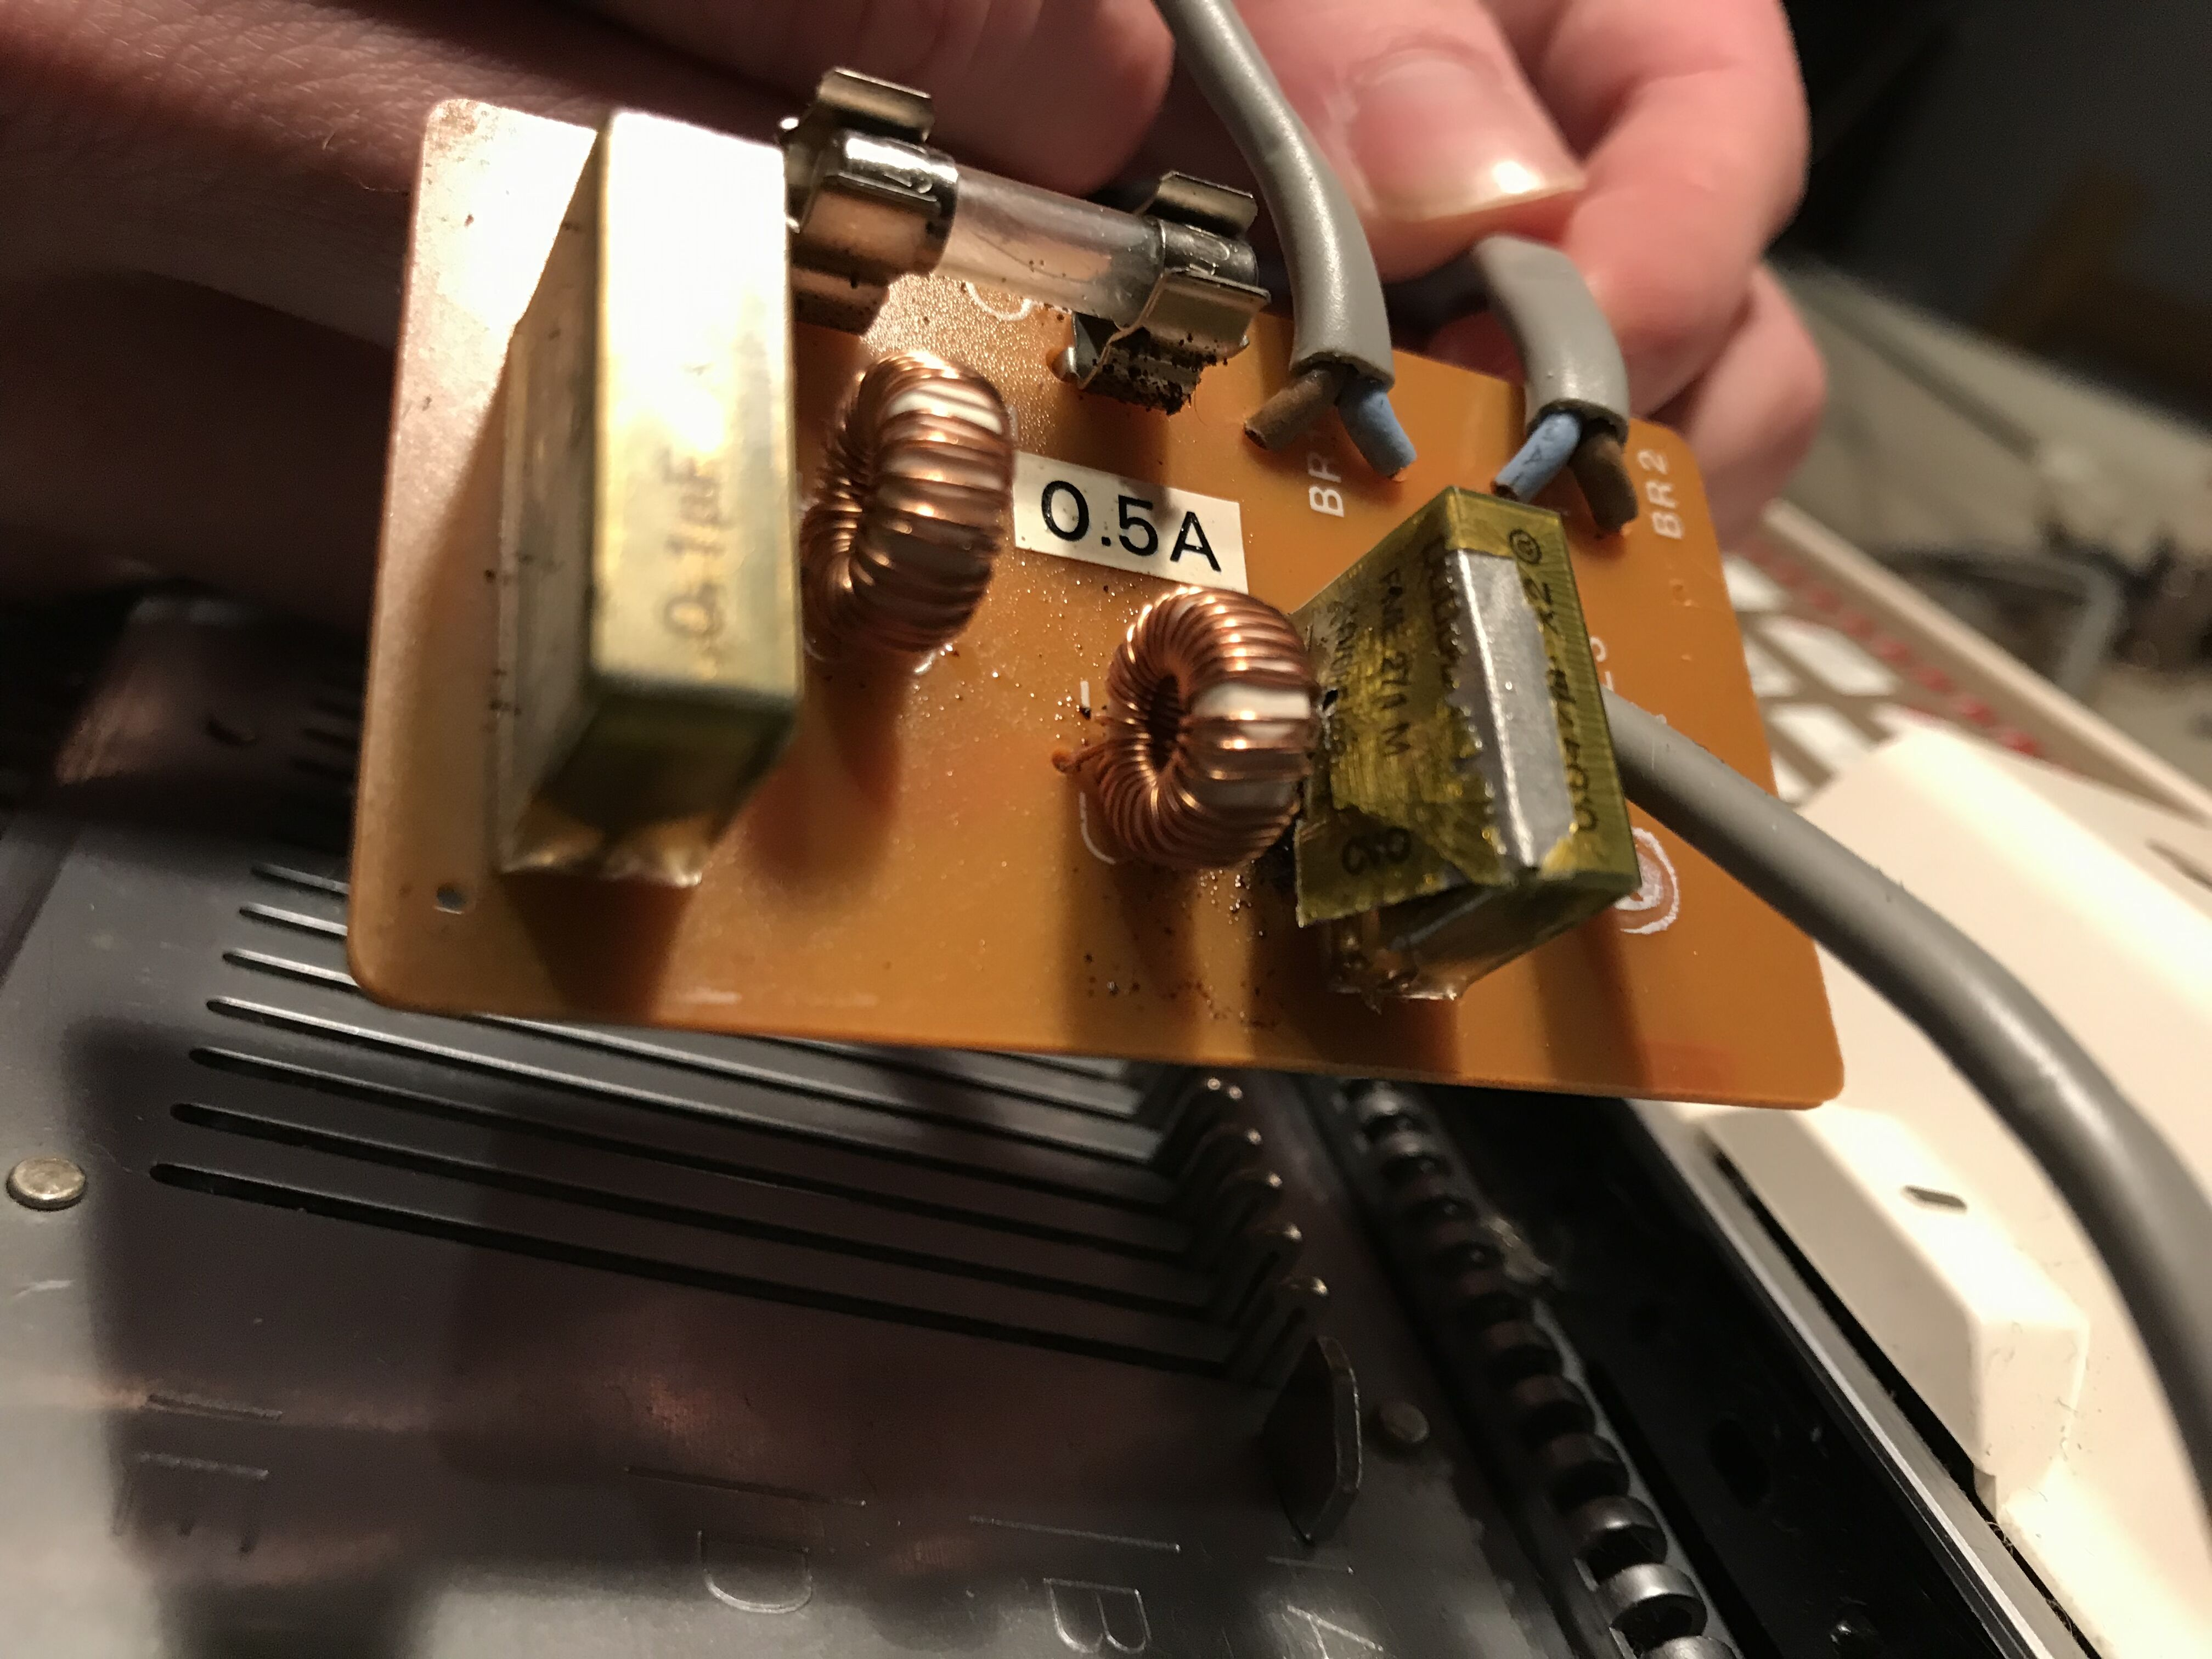
\includegraphics[width=0.7\textwidth]{./images/exploded-capacitor.png}
        \caption{fubar}
    \end{figure}
\end{frame}

\begin{frame}{the brother kh-940}
    \begin{itemize}%[<+->]
        \item technical documentation
        \item photos
        \item the data interface
    \end{itemize}
\end{frame}

\begin{frame}{the different projects}
    \begin{itemize}
        \item knitt
        \begin{itemize}
            \item the machine
        \end{itemize}

        \item michael
        \begin{itemize}
            \item the usb driver
        \end{itemize}

        \item devon
        \begin{itemize}
            \item one UI to rule them all
        \end{itemize}
      \end{itemize}
\end{frame}

\end{document}
